\chapter{Verification of Three Key Establishment Protocols}
\label{chp:analysis}


\section{Modelling Security Claims}

As mentioned in Section \ref{sec:attributes}, key establishment schemes desire certain security properties. In the verification of the security protocols of this thesis, the following properties are verified: \emph{Entity authentication}, \emph{Implicit key authentication}, \emph{Explicit key authentication}, \emph{Known-key secrecy}, \emph{Key control}, and \emph{Secrecy of key}. As mentioned in Section \ref{sec:attributes}, symmetric key establishment schemes are not resilient against \gls{kci} attacks, and do not provide forward secrecy. %Therefore, these properties are nevertheless included in the models as \gls{sakes} supports a lightweight version of public-key cryptography utilizing session keys.

\paragraph{Entity authentication:} Entity authentication between nodes corresponds to the security claim \texttt{Alive}, and can also be verified through stronger claims such as \texttt{Weakagree}. MORE %MOREOROEROEROER

\paragraph{Implicit key authentication} Implicit key authentication is modelled through the settings of the adversary compromise model described in Section \ref{sec:adversary}. This property is modelled by allowing the adversary to obtain the long-term keys and impersonate anyone except for the nodes that are supposedly establishing keys.

\paragraph{Explicit key authentication} Is achieved when the protocol satisfied both implicit key authentication and key confirmation. This is modelled through the security claim for \emph{non-injective agreement} denoted as \texttt{ni-agree}, but can also be modelled by using \texttt{running} and \texttt{commit} claims.

\paragraph{Known-key security} By revealing session keys to the adversary after usage (i.e. the session key is expired, and will never be used again) known-key security can be modelled. This is done by setting the \emph{Session-key reveal} rule in the adversary compromise model.

\paragraph{Key control} Scyther has no support for verifying key control. Therefore, this security property has to verified by hand. 

\paragraph{Secrecy of key} To model a key (or any other property) as secret, the \texttt{secrecy} claim is used in Scyther.

\paragraph{Forward secrecy} Both \gls{pfs} and \gls{wpfs} are related to active adversaries, and is modelled through the adversary compromise model, where rules for leaking the long-term private key which the session keys are derived from can be enabled.

\paragraph{Key compromise impersonation} \gls{kci} is also a property related to an active adversary, and is therefore available through the adversary model where the adversary can be allowed to obtain the long-term private key of the actors.


\section{Formal Security Analysis of APKES}

The \gls{apkes} protocol is modelled using Scyther, and can be viewed in its entirety in Appendix \ref{app:apkes}. The protocol is modelled as two roles, the initiator $A$ and the responder $B$, agreeing upon a pairwise key through the message exchange that is presented in Figure \ref{fig:apkes-handshake}. There is not specified any concrete type of pluggable scheme (i.e. the scheme where \gls{apkes} obtains the shared secret between two nodes), hence we assume that whatever scheme is used is secure. In the model, the shared secret obtained from the pluggable scheme has modelled by using Scyther's built-in support for shared symmetric keys, where the two nodes $A$ and $B$ initially share a symmetric key.

\subsection{Security Claims}

By taking starting point in the protocol specification from Section \ref{subsec:apkes-spec} and the alleged security properties from Section \ref{subsec:apkes-prop}, the protocol is modelled as a \gls{spdl}-script, which can be verified by Scyther. Listing \ref{lst:claims-u-apkes} describes the various security claims that is chosen for $A$.


\begin{lstlisting}[caption={Security claims for role A in APKES.}, label={lst:claims-u-apkes}]
		claim_A1(A, Alive);
		claim_A2(A, Weakagree);
		claim_A3(A, Niagree);
		claim_A4(A, Nisynch);
		claim_A5(A, Commit, V, Ru);
		claim_A6(A, Secret, PairwiseKey);
\end{lstlisting}

In Listing \ref{lst:claims-v-apkes} below, the security claims for the role $B$ in \gls{apkes} are stated. Compared to the claims for $A$, $B$ does not contain the \texttt{Commit} claim, as the \texttt{Running}, \texttt{Commit} approach is used in role $A$ to provide agreement over the nonce $Ru$. \gls{apkes} states that the $R_A$ value has to be checked whether or not it has been tampered with, before the pairwise key can be derived at the initiating side. This can be verified by modelling the protocol to agree upon the $R_A$ value during the protocol execution, and committing to this.

\begin{lstlisting}[caption={Security claims for role B in APKES.}, label={lst:claims-v-apkes}]
		claim_B1(B, Alive);
		claim_B2(B, Weakagree);
		claim_B3(B, Niagree);
		claim_B4(B, Nisynch);
		claim_B5(B, Secret, PairwiseKey);
\end{lstlisting}


\subsection{Adversary}

In the description of \gls{apkes}, no specific adversary is mentioned. If we assume that such a protocol would be used for key establishment in \gls{6lowpan} networks, which are potentially deployed in hostile areas, we can assume that the adversary would be able to monitor all messages sent over the network. As \gls{apkes} does not utilize any session keys, but rather agreeing upon a fixed long-term key, we model the adversary in a Dolev-Yao way without giving it any active capabilities other than being able to obtain the long-term keys of nodes not participating in the current key establishment process. 

\subsection{Results}

Figure \ref{fig:apkes-verified} shows the verification result from running the model of \gls{apkes} through Scyther in the presence of the adversary described above. Scyther was able to perform an unbounded verification of the model, with only one possible trace from the characterization process, effectively meaning that there is only one possible way to execute the protocol. \gls{apkes} provides verifiable entity authentication, explicit key authentication, and holds the non-injective synchronization property, which means that every message in protocol was executed as expected, even in the presence of an adversary. 

\begin{figure}[h]
	\centering
	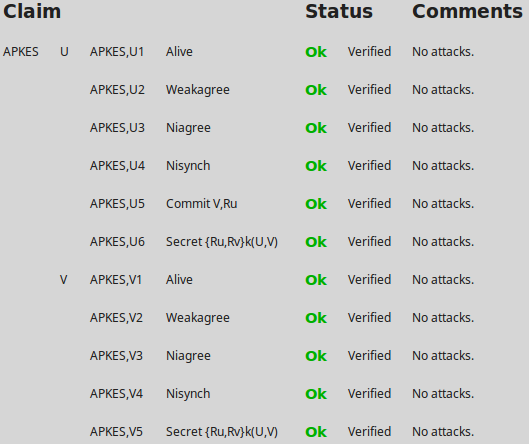
\includegraphics[scale=0.92]{apkes-verified.png}
	\caption{Result of verifying APKES' security claims using Scyther.}
	\label{fig:apkes-verified}
\end{figure}




\section{Formal Security Analysis of AKES}



\subsection{Security Claims}

\subsection{Adversary}





\section{Formal Security Analysis of SAKES}

\subsection{Security Claims}

\subsection{Adversary}


